% % % % % % % % % % % % % % % % % % % % % % % % % % % % % % % % % % % % %
% Chapter: Experiment 3
% % % % % % % % % % % % % % % % % % % % % % % % % % % % % % % % % % % % %
\chapter{Experiment 3: Automatic value generation}
\label{cpt:experiment3}
In the second experiment (\autoref{cpt:experiment2}), we found that the property
definition for using division with the \textit{Money} type wasn't clear enough
in that it couldn't be satisfied the way how it was specified. In this
experiment we aim to improve this, by updating the existing definition such that
the property can now be checked.\\
\\
A limitation in the second experiment was that the value generation was not
very dynamic when new property definitions were being added. It should be possible to add
additional properties to the specification, such that these properties are being tested
automatically by the test framework. To do this, the value generator should be
updated too, such that it uses the preconditions in the event definitions to
determine the input values. Additional properties can then be added to test
the generator.\\
\\
In this experiment we will use the updated version of the generator, in which
the precision errors that were found in the first experiment are fixed.
This is done, such that we can focus on possible additional errors that might occur.

% % % % % % % % % % % % % % % % % % % % % % % % % % % % % % % % % % % % %
% Section: Method
\section{Method}
The property definitions of \textit{Division} is being updated for this experiment because
the first definition did not take the division problem into account. There was
also no definition for rounding the value, as the value was expected to hold the
exact value. We will update the definition by implementing a rounding function,
such that these properties can be tested by the test
framework.\\
\\
Besides updating the property definitions for \textit{Division}, additional
property definitions are being added to test more of the generator. However, as
we have seen in the second experiment, the values generator was not very
dynamic. Which resulted in that it had to be modified in case an implicative
property is being added to the specification. This is the second thing that
should be improved, such that additional (implicative) properties do not require
modifications to the values generator.

% % % % % % % % % % % % %
% Subsection: Updating property definitions
\subsection{Updating property definitions}
\pinfo{Round method}
Initially, there were only 2 property definitions that were using division,
which both are being updated. In order to check for the values such that the
property definition can be used, we implement a \code{round()} method in the
\textit{Rebel} specification. This \textit{round} method is intended to return a
value which can be used to define the expected behaviour when using division
with the \textit{Money} type.\\
\\
\pinfo{Defining, updating and adding more}
In addition to updating the existing properties that are using division, more
properties can be added which were not defined earlier. Additional properties
might also lead to additional bugs that the test framework can detect. For
example, properties of inequality when using division, as the ones that were
defined for division only used equality. We add more properties to the existing set of property definitions that we
defined for \textit{Rebel}: Properties for division, multiplication, additivity and subtraction.\\
\\
The additional property definitions for division,
multiplication, additivity and subtraction fall under the
``Properties of equality and inequality'' category and are defined in
\autoref{ssct:properties_definitions_additionalproperties}, along with the
updated definitions. To sum up, the updated and added property definitions are:
\textit{divisionEquality}, \textit{divisionInequality},
\textit{additiveEquality}, \textit{additiveInequality},
\textit{subtractiveEquality}, \textit{subtractiveInequality},
\textit{multiplicativeEquality} and \textit{multiplicativeInequality}.\\
\\
\pinfo{Round method implementation + why}
Some properties using division are now using the \code{round()} method in its
definition. \textit{Rebel} does not provide a way to round a value, which is why
we need to define the function in the specification. In \textit{Rebel}, a
function is defined as an expression that is being executed whenever the
function is being called. Unfortunately, there is currently no way in
\textit{Rebel} to write down the \textit{Scala} implementation of this
\textit{round} function. As a workaround, we define the implementation as a
\textit{String} and modify the generator such that the content of the
\textit{String} (removing the quotes) will be the implementation of the
function. The \textit{round} method rounds the \textit{Money} value to a maximum
of 4 decimals.\\
\\
In \textit{Java} (and thus in \textit{Scala}), there are different rounding
methods available. These consist of the rounding modes described in the IEEE 854
standard and additional rounding modes as described
in~\cite{cowlishaw2003decimal}. The fifth decimal in our \textit{round()} method
is being rounded by using the ``HALF\_UP'' rounding mode
(described in~\cite{cowlishaw2003decimal}). We chose for the ``HALF\_UP'' as this is more in line with
our expectations and this mode is perhaps the most commonly used rounding mode when rounding
financial numbers. However, we also analyse the effects of using some of the other available rounding modes. The implementation of the \textit{round()} method in the
\textit{Rebel} specification is shown in
\autoref{lst:experiment3_rebel_round_implementation}.
% Listing
\begin{sourcecode}[!ht]
\begin{lstlisting}[language=Rebel]
function round(money: Money): Money =
    "money.currency(money.amount.setScale(4, RoundingMode.HALF_UP))";
\end{lstlisting}
\caption{The \textit{round()} function in the \textit{Rebel} specification.}
\label{lst:experiment3_rebel_round_implementation}
\end{sourcecode}
\FloatBarrier\noindent
% End listing

% % % % % % % % % % % % %
% Subsection: Improving dynamicallity
\subsection{Improving dynamicallity}
\pinfo{Using preconditions}
The additional properties that are being added also use implication in their
definitions. In the second experiment (\autoref{cpt:experiment2}), the value
generator was not dynamic enough in that it requires modifications to the
implementation for each implicative property that is being added. In this
experiment, we aim to improve this, by using the defined preconditions to
determine the input values.\\
\\
A custom value generator is being created that uses the preconditions to determine the
input values. Note that this can be seen as an update to the earlier value generator that was
created in \autoref{cpt:experiment2}. This value generator parses the
preconditions and intends to generate values based on these conditions. Since
the expressions inside the preconditions can become complex, we focus on
a limited version of it. Limited in the sense that we support all of the properties that we defined in \autoref{cpt:properties}, but other expressions that were not used in our definitions might be unsupported.\\
\\
Most properties are using single variables in its precondition statements. Some
are using expressions on the left-hand or right-hand side of a statement, but
not on both sides. The value generator that we implement will not support using
expressions on both the left-hand and right-hand side, as generating values
matching the condition can result in complex formulas. With expressions, we mean a
combination of operators with literals and variables. Instead, the value generator requires having at least a variable on one side of the
expression.\\
\\
The code to generate the tuples of input values is shown in
\autoref{lst:experiment3_value_generation_code}. We can separate this process
into the following steps:
\def \valueGeneratorStepOne{Initialize value generation data (\hyperref[lst:experiment3_value_generation_code]{Line 7})}
\def \valueGeneratorStepTwo{Traverse and handle statements (\hyperref[lst:experiment3_value_generation_code]{Line 9-13})}
\def \valueGeneratorStepThree{Generate values for remaining, unassigned, variables (\hyperref[lst:experiment3_value_generation_code]{Line 15-18})}
\def \valueGeneratorStepFour{Add values to resulting list (\hyperref[lst:experiment3_value_generation_code]{Line 21})}
\begin{enumerate}
  \item \valueGeneratorStepOne
  \item \valueGeneratorStepTwo
  \item \valueGeneratorStepThree
  \item \valueGeneratorStepFour
\end{enumerate}
% Listing
\begin{sourcecode}[!ht]
\begin{lstlisting}[language=Rascal]
public list[list[Expr]] genValues(str eventName, Preconditions? preconditions, list[Parameter] transitionParams, int amount) {
    println("\> Generating values for event <eventName>");

    list[list[Expr]] valueList = [];
    for (int i <- [0..amount]) {
        calculatedParams = (); // Clear old data
        paramGenData = ("<p.name>" : <p.tipe, -9999.00, 9999.00, true> | p <- transitionParams);

        // Calculating
        for(/Statement s <- preconditions) {
            <lhs, rhs, operator> = extractStatementData(s.expr);
            handleConditionStatement(operator, lhs, rhs);
        }

        // Check whether all are determined, if not, determine those using the randomValueProps data
        for (Parameter p <- transitionParams, !calculatedParams["<p.name>"]?) {
            calculatedParams["<p.name>"] = calculateExpression(p.name);
        }

        // Add to list
        valueList += [[getExprForVar("<p.name>") | p <- transitionParams]];
    }
    return valueList;
}
\end{lstlisting}
\caption{Code to generate the list of input values for an event.}
\label{lst:experiment3_value_generation_code}
\end{sourcecode}
\FloatBarrier\noindent
% End listing
%
In the following sections we describe each step in detail.

% Initialize value generation data for each variable
\subsubsection{1. \valueGeneratorStepOne}
To generate a single value, some data is being held to keep track of the
conditions which the generated value should fulfil. These
conditions are the minimum value, the maximum value and whether the zero value
is allowed. Additionally, the result type of the variable is stored, used when
generating the final value. This data is stored in a tuple and called
\textit{RandomValueProps} by using an \textit{alias} in \textit{Rascal}. This
definition is shown in
\autoref{lst:experiment3_alias_definition_randomvalueprops}.
% Listing
\begin{sourcecode}[!ht]
\begin{lstlisting}[language=Rascal]
// Minimum: including. So: if 0, then 0 can be a result value when determining it random.
// Maximum: including. So: if 10, then 10.00 is max result value when determining random.
alias RandomValueProps = tuple[Type valueType, real min, real max, bool allowZero];
\end{lstlisting}
\caption{The definition of \textit{RandomValueProps} in \textit{Rascal}.}
\label{lst:experiment3_alias_definition_randomvalueprops}
\end{sourcecode}
\FloatBarrier\noindent
% End listing
The value generator initializes the \textit{RandomValueProps} for each input
variable. Setting the minimum and maximum value to a default value and allowing
zero by default.

% Traverse statements in the precondition block and handle these based on the expression
\subsubsection{2. \valueGeneratorStepTwo}
Each statement in the preconditions block is being checked. The
\textit{handleStatement()} method handles each statement. The actions done by
this method depend on the operators used in the statement that is being
handled.\\
\\
In case of an expression that only contains variables and uses equality
(for example, \textit{x == y}), the value generator assigns a random value to
\textit{x} and assigns the same value to \textit{y}. In case of inequality
(for example, \textit{x $<$ y} or \textit{x $>$ y}), the value generator also assigns a random value to
\textit{x} and adjusts the minimum or maximum bounds of the \textit{y} value
such that it satisfies the condition.\\
\\
In case there is an expression on one side (for example, \textit{x * y == z}),
the expression will be evaluated first. In this case, random values will be
assigned to \textit{x} and \textit{y}. Next, the expression can be evaluated and
the result of that is being assigned to \textit{z}. The same is done with
inequality relations, but then the minimum or maximum bounds are being set based
on the operator.\\
\\
As mentioned earlier, having expressions on both the left-hand and the
right-hand side of the expression is unsupported. The \textit{handleStatement()}
method will throw an error in case this happens.

% Generate values for yet unassigned variables
\subsubsection{3. \valueGeneratorStepThree}
When handling each expression, some variables already get an assigned value.
However, some variables might only have their \textit{RandomValueProps} updated
but do not have an assigned value yet. In this step, the variables that do not
have an assigned value, are being assigned a value based on their
\textit{RandomValueProps}.

% Add values to resulting list
\subsubsection{4. \valueGeneratorStepFour}
The values that have been determined are being added to the list of generated
input values. In the end, the list is being returned, containing all the
generated input values that match the preconditions of the event.

% % % % % % % % % % % % % % % % % % % % % % % % % % % % % % % % % % % % %
% Section: Results
\section{Results}
% - Run, tests succeed (hopefully)
Running the test framework with the addition of the properties defined in
(\autoref{ssct:properties_definitions_additionalproperties}) results in no
additional failing tests compared to the first experiment. Remember that the
test framework is run with the generator in which the precision problems related
to the \textit{Money} type are fixed (otherwise there would be additional failing tests,
due to the precision problems).\\
\\
There are still 3 failing tests in total, which are not fixed in the generator
yet. These bugs have already been reported in the first experiment and thus are
not new in this experiment.

% % % % % % % % % % % % % % % % % % % % % % % % % % % % % % % % % % % % %
% Section: Analysis
\section{Analysis}
% - Test succeeding provided rounding
% - Case of rounding down, it fails (bigger number shows difference)
% - > Thus probably division does this too usually. FLooring causes difference
The tests are succeeding due to the implementation of the \textit{round()}
method. It rounds the value of \textit{Money} to 4 decimals using the
``HALF\_UP'' rounding mode. The number 4 is chosen here to ensure that the
property definitions should hold up to a precision of 4 decimals when using the
round method. However, this can be modified in case a bigger precision is
preferred. Changing the precision number to 6 or 8 decimals does not change the
results when looking at the number of failing tests. Also, changing the rounding
mode to ``DOWN'' does not affect our results. Although, when using a bigger precision in
combination with another rounding mode, such as ``FLOOR'' or ``TOP'', can result
in some failing tests. This is being caused by an edge case in which the
difference would be slightly off between the two values.\\
\\
We stay with the implementation of ``HALF\_UP'' as rounding mode, as this is
more in line with our expectations and this mode is perhaps the most commonly
used rounding mode when rounding financial numbers. This rounding mode is also
described as a
``requirement for many financial calculations''~\cite{cowlishaw2003decimal}. One
might want to use the ``DOWN'' rounding mode because a bank would prevent losing
money because of this rounding issue. When this is the case, it can always be
changed in the \textit{Rebel} specification when needed, we stick with
``HALF\_UP'' as rounding mode.\\
\\
% - Adding properties didn't require a change in the value generator anymore
For this experiment, additional property definitions have been added to test the
generator. The value generator now determines the values based on the
preconditions of the properties. Thus the additional properties used in this
experiment did not require more effort than writing these down in the \textit{Rebel}
specification. Compared to the second experiment (\autoref{cpt:experiment2})
this is a huge improvement, as it does not require the developer to modify the
value generator when implicative properties are being added.\\
\\
\pinfo{BMC possibility, tested. But not working}
Another way how the values could be generated is by using existing solvers.
Since the \textit{Rebel} toolchain already makes
use of a bounded model checker to check a specification, this could be used to
translate an expression and retrieve values for which the condition holds.\\
\\
\pinfo{Checked using Z3, but returns same values all the time}
We have looked into this, by using the \textit{Z3} solver. However, the solver
always returns the same number when executing it multiple times. Which means
that the 100 values that we would ask from the generator, will be exactly the
same. A workaround would be to then add the number that was received earlier as
an additional constraint, such that 100 unique values are being retrieved. But
the problem still remains, as executing the same script multiple times will
result in the same values. Another possibility would be to change the seed of
the random generator that is being used to generate the values, resulting in
different values, however, then a random seed should be used each time the
solver is being run to make the generated values unique. In order to integrate
the solver with the test framework, the value generator has to be changed.\\
\\
Checking a \textit{Rebel} specification by using the existing tool chain can already take up some time. Which is probably
related to the translations that have to be done and actually running the
solver. We have not measured the exact duration of each step in this case, but
we expect that generating 100 random input values by using this existing implementation in the tool chain
requires some time. Resulting in a overall run time increase for the test
framework.\\
\\
Other solvers might work better for this approach, but these still require an
update to the values generation part of the test framework to integrate with
such solvers. We stick with our own implementation. The properties that are defined until now can be tested by the test framework automatically with this implementation, as well as additional property definitions in case these are supported by this implementation.

% % % % % % % % % % % % % % % % % % % % % % % % % % % % % % % % % % % % %
% Section: Evaluation criteria
\section{Evaluation criteria}
\pinfo{Not huge diff in coverage. But added props}
The coverage in this experiment is almost the same as in the second experiment.
The implicative properties are being checked in the same way. In this
experiment, additional properties were added. The total test coverage is 88,28\%
(which is 0,42\% lower than the second experiment), shown in
\autoref{fig:experiment3_eval_e3}. This shows that adding additional properties
do not increase or decrease the test coverage in big amounts. The small
percentage loss could be related to the fact that we do not check the
\textit{else} clauses of the implicative properties.
% Figure
\begin{figure}[!ht]
%\frame{
	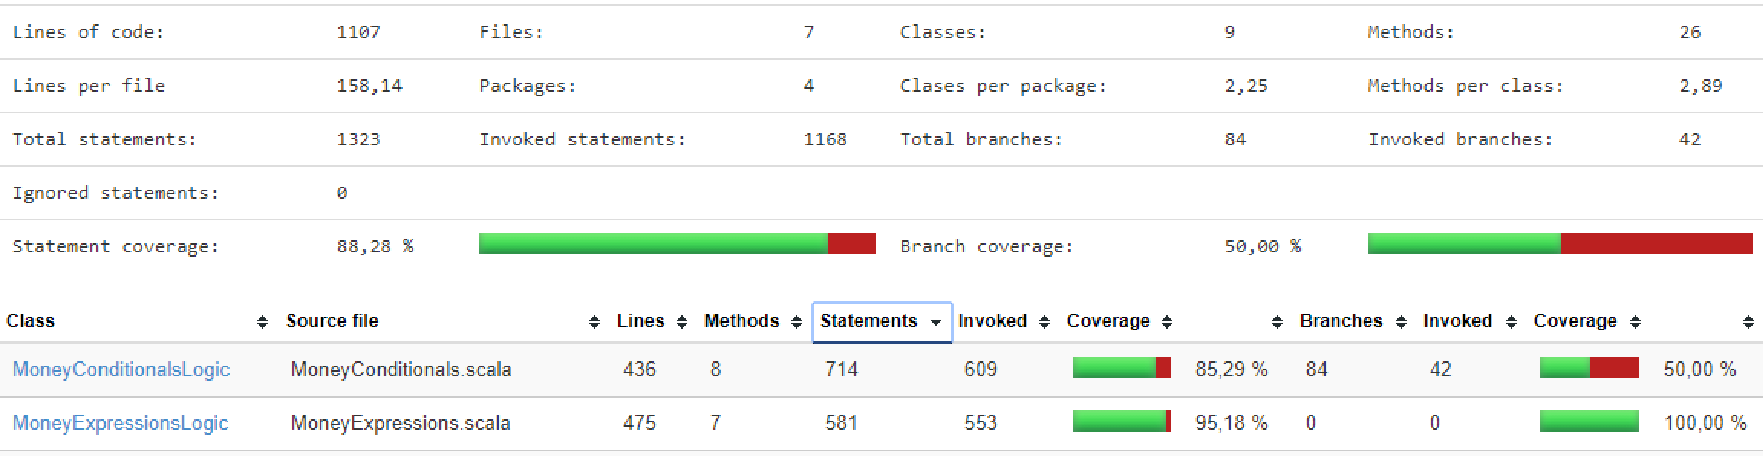
\includegraphics[width=\linewidth]{figures/eval_e3}
%}
\caption{Test coverage report of the third experiment}
\label{fig:experiment3_eval_e3}
\centering
\end{figure}
\FloatBarrier\noindent
% End figure
%\pinfo{Branch coverage still 50\%}
The branch coverage is still reported to be 50\%, while the number of branches
has been increased. This is correct, as the additional properties are using the
implication symbol, which is being translated to if-else statements. This
introduces these extra branches. As described before, we do not intend to check
the else-clause but are more interested in checking the if-clause.\\
\\
% - No extra bugs found
\pinfo{No 'extra' bugs found}
Unfortunately, no additional bugs have been found in this experiment. Additional
properties were being used in this experiment compared to the other experiments,
but these did not reveal more bugs. The implicative properties are checked
in the same way as in the second experiment, but the values are now generated
based on the preconditions of the event definitions in the \textit{Rebel}
specification.\\
\\
%   > but increased dynamicallity. We have shown that additional properties can now be added to check, without needing to update the test framework
The properties that have been added did not require changes in the value
generator anymore. Instead, these only had to be written down in the \textit{Rebel}
specification. The test framework automatically determines the input values for it.
This is an improvement compared to the second experiment, as there it would be
required to update the value generator whenever an implicative property is
added. There are still some limitations on the value generator, for example, it
does not support complex expressions as preconditions. This is also not needed
for the current set of property definitions and might or might not be needed in
the future. Because of this, we leave the implementation for supporting complex
expressions in the value generation as future work.

% % % % % % % % % % % % % % % % % % % % % % % % % % % % % % % % % % % % %
% Section: Conclusion
\section{Conclusion}
This experiment focused on improving the value generation, such that it is not
required to update the test framework whenever an implicative property is being
added to the \textit{Rebel} specification. The value generator now uses the
statements in the precondition block to determine the input values, which hereby
satisfy the preconditions. We have shown that this increased the dynamicallity
by adding additional properties. Adding these properties to the test
framework was only a matter of translating those property definitions to \textit{events} in the
\textit{Rebel} specification.\\
\\
This experiment did not reveal extra bugs in the generator, but we have shown
that adding more property definitions does not require an update to the test
framework when it comes to implicative properties. However, there are still some
limitations when it comes to the value generation. One of the limitations is
that it does not work with complex expressions as preconditions. The value
generator will throw an exception when an expression is given that is
unsupported.

% % % % % % % % % % % % % % % % % % % % % % % % % % % % % % % % % % % % %
% Section: Threats to validity
\section{Threats to validity}
In \autoref{cpt:testmechanics} and \autoref{cpt:experiment2} we described the threat concerning generating incorrect input values. In this experiment we brought changes to the way how these input values are being determined. However, the threat still remains as the current implementation could contain some errors too. When running the test framework, we haven't encountered issues with this, other than the one described in \autoref{cpt:experiment2}.



% - Implementation error in our generator. However, we generate random values every run. (unlike Z3)
% > Running multiple times might give a fault-positive. High probability this is caused by the random operation that is done on the input values. This is a threat that came forth from experiment 2, and still exists here. - (Using > or < with 0 0 0 can happen because of this)

% - Existing approaches are available too, we only checked the Z3. But SageMath or others are possibilities too. However, this requires us to make such a tool compatible with the test framework. Our own implementation has shown to work for the properties we have defined. In case of more complex properties, it might be more useful to use another tool to determine these values.

% More reliable solving. Checked but not working as expected. Which is why we did our own generator
% \subsubsection{Using existing solvers}



%
%\pinfo{Other possibilities, future work}
%There are other solvers available too, or other methods to generate values that
%match the condition. It would be useful to make the test framework more dynamic
%when such properties are being used.
